\chapter{Definitions and datasets\label{chap::def}}

Trees are partitioned into hierarchical elements with definitions that may vary between Forest Inventories and datasets (\eg Fig. \ref{fig::partition}).

\begin{figure*}[h]
	\centering
	\begin{tikzpicture}
	%% Level 0
	\node (orig) at (0, 0) {Whole tree};
	
	%% Level 1
	\node[below right = of orig] (belowground) {Below-ground};
	\node[above right = of orig] (aboveground) {Above-ground};
	
	%% Level 2
	\node[above right = of aboveground] (stem) {Main stem};
	\node[right = of aboveground] (lat) {Lateral};
	\node[below right = of aboveground] (fol) {Foliage};
	
	\node[right = of belowground] (root) {Root};

	%% Level 3
	\node[above right = of stem] (stemtop) {Stem top};
	\node[right = of stem] (bole) {Bole};
	\node[below right = of stem] (stump) {Stump};

	\node[below right = of lat] (lbranch) {Large branches};
	\node[above right = of lat] (sbranch) {Small branches};

	\begin{scope}[on background layer] % From background library
		% \fill[lightGrey] (2.735294,0) rectangle (6,6);
		\node[fit=(belowground)(aboveground), fill = lightGrey, inner sep=5mm] {};
	\end{scope}

\end{tikzpicture}
	\caption{Hierarchical elements of trees, figure inspired by \cite{Gschwantner2009} \label{fig::partition}}
\end{figure*}

In our case, the tree data were collected from several institutions, at different periods, and with varying levels of detail regarding recorded tree components:

\begin{marginfigure}
	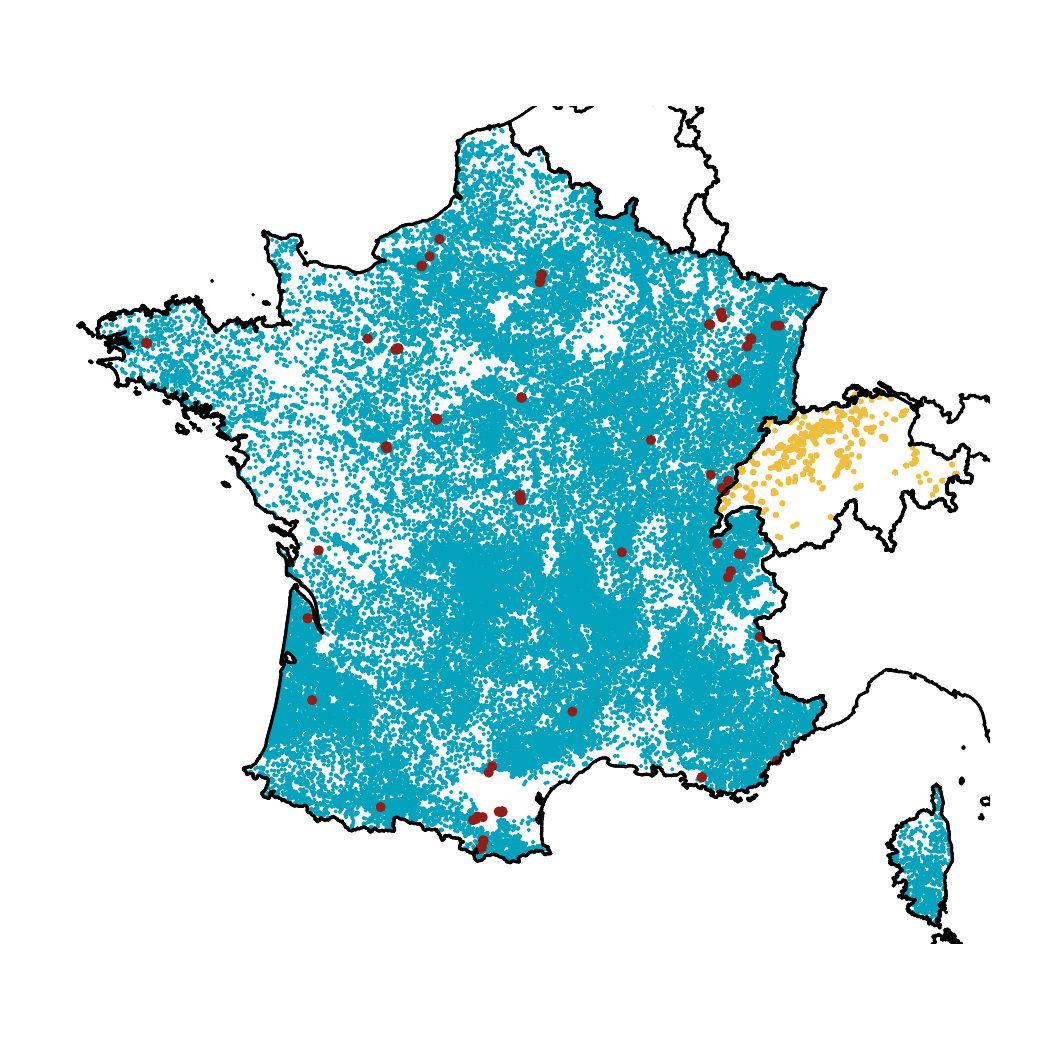
\includegraphics[width = \marginparwidth]{./Figures/map.png}
	\caption{Plot location for French \NFI, Emerge, and Swiss dataset.\label{fig::map}}
\end{marginfigure}

\begin{enumerate}
	\item `Protocole Oudin' dataset -- Preserved by INRAE and covering the period 1930--1980 (shown in red in Fig. \ref{fig::map}). This dataset includes measurements of bole volume, large branches, and small branches. Hereafter, it is referred to as `Emerge', after the 2008 digitisation project of the same name \parencite{Deleuze2013}.
	\item Experimental Forest Management Project dataset (EFM) -- Described by Didion et al. (2024) and covering the period 1888--1974 (shown in yellow in Fig. \ref{fig::map}). It includes measurements of bole volume, large branches, and small branches.
	\item French National Forest Inventory (\NFI) -- Data collected between 1988 and 2007 (shown in blue in Fig. \ref{fig::map}). Earlier data (before 1988) recorded diameter instead of circumference and are discarded in this study. This dataset contains measurements of bole volume, following the \NFI{} protocol (less detailed than Emerge and EFM).
	\item `Office National des Forêts (ONF)' -- Data collected with protocols from 1972 and from 1983. So far, these data are not used due to the absence of geographic coordinates.
	\item Institut Technologique Forêt, Cellulose, Bois-construction, Ameublement (FCBA) -- Data available but not yet used for above-ground volume estimation.
	\item Institut pour le Développement Forestier (IDF) -- The R\&D branch of the Centre National de la Propriété Forestière (CNPF). Data not used.
\end{enumerate}

The terminology follows that of \cite{Gschwantner2009} (see Figs. \ref{fig::partition} and \ref{fig::ign_tree}) to ensure consistency in wording across the different datasets:

\begin{marginfigure}
	\begin{tikzpicture}
	\node (tree) at (0, 0) {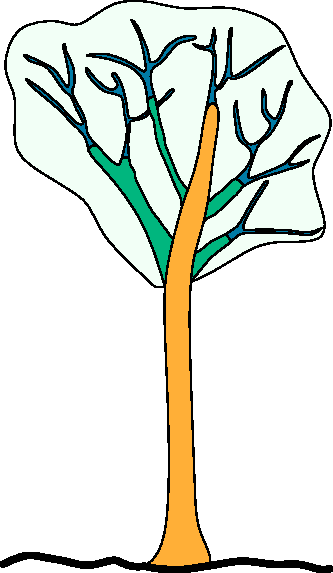
\includegraphics[width=\marginparwidth]{./Figures/ign_tree.pdf}};
	\matrix[below = -0.2cm of tree] {
		\node [draw, shape = rectangle, fill = egyptYellow, label = right:Bole] {}; \\
		\node [draw, shape = rectangle, fill = egyptGreen, label = right:Large branches] {}; \\
		\node [draw, shape = rectangle, fill = egyptBlue, label = right:Small branches] {}; \\
	};
\end{tikzpicture}
	\caption{Scheme of tree components.\label{fig::ign_tree}}
\end{marginfigure}

\begin{itemize}
	\item Main stem: The stem of a tree is the above-ground part of the main (off) shoot with apical dominance
	\begin{itemize}
		\item Stem top: topmost part of the stem from an over-bark base-diameter of \qty{7}{\centi\metre} (French \NFI) to the stem tip
		\item Bole: above-ground part of the stem between stump and the stem top
		\item Stump: above-ground base part of the stem which would remain after a tree was cut under normal felling practices
	\end{itemize}
	\item Lateral parts:
	\begin{itemize}
		\item Large branches: portion of the above-ground lateral parts with a diameter of more than or equal to \qty{7}{\centi\metre} (French \NFI)
		\item Small branches: portion of the above-ground lateral parts with a diameter of less than \qty{7}{\centi\metre} (French \NFI)
	\end{itemize}
\end{itemize}

\begin{marginfigure}
	\centering
	% Created by tikzDevice version 0.12.6 on 2025-10-06 15:09:30
% !TEX encoding = UTF-8 Unicode
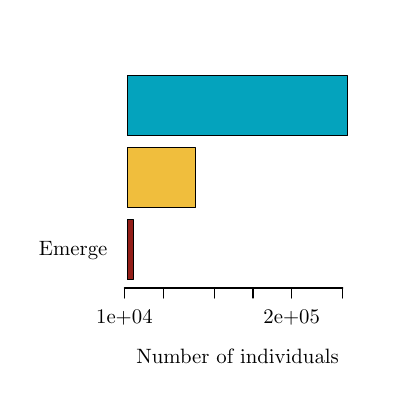
\begin{tikzpicture}[x=1pt,y=1pt,scale=0.6]
\definecolor{fillColor}{RGB}{255,255,255}
\path[use as bounding box,fill=fillColor,fill opacity=0.00] (0,0) rectangle (216.81,216.81);
\begin{scope}
\path[clip] (  0.00,  0.00) rectangle (216.81,216.81);
\definecolor{drawColor}{RGB}{0,0,0}
\definecolor{fillColor}{RGB}{147,30,24}

\path[draw=drawColor,line width= 0.4pt,line join=round,line cap=round,fill=fillColor] ( 60.00, 64.92) rectangle ( 63.54,101.09);
\definecolor{fillColor}{RGB}{240,190,61}

\path[draw=drawColor,line width= 0.4pt,line join=round,line cap=round,fill=fillColor] ( 60.00,108.32) rectangle (101.25,144.49);
\definecolor{fillColor}{RGB}{4,163,189}

\path[draw=drawColor,line width= 0.4pt,line join=round,line cap=round,fill=fillColor] ( 60.00,151.72) rectangle (192.81,187.89);
\end{scope}
\begin{scope}
\path[clip] (  0.00,  0.00) rectangle (216.81,216.81);
\definecolor{drawColor}{RGB}{0,0,0}

\node[text=drawColor,anchor=base east,inner sep=0pt, outer sep=0pt, scale=  0.75] at ( 48.00, 79.56) {Emerge};

\node[text=drawColor,anchor=base east,inner sep=0pt, outer sep=0pt, scale=  0.75] at ( 48.00,122.96) {\EFM};

\node[text=drawColor,anchor=base east,inner sep=0pt, outer sep=0pt, scale=  0.75] at ( 48.00,166.36) {\NFI};
\end{scope}
\begin{scope}
\path[clip] (  0.00,  0.00) rectangle (216.81,216.81);
\definecolor{drawColor}{RGB}{0,0,0}

\node[text=drawColor,anchor=base,inner sep=0pt, outer sep=0pt, scale=  0.75] at (126.41, 14.40) {Number of individuals};
\end{scope}
\begin{scope}
\path[clip] (  0.00,  0.00) rectangle (216.81,216.81);
\definecolor{drawColor}{RGB}{0,0,0}

\path[draw=drawColor,line width= 0.4pt,line join=round,line cap=round] ( 58.25, 60.00) -- (189.79, 60.00);

\path[draw=drawColor,line width= 0.4pt,line join=round,line cap=round] ( 58.25, 60.00) -- ( 58.25, 54.00);

\path[draw=drawColor,line width= 0.4pt,line join=round,line cap=round] ( 81.56, 60.00) -- ( 81.56, 54.00);

\path[draw=drawColor,line width= 0.4pt,line join=round,line cap=round] (112.37, 60.00) -- (112.37, 54.00);

\path[draw=drawColor,line width= 0.4pt,line join=round,line cap=round] (135.67, 60.00) -- (135.67, 54.00);

\path[draw=drawColor,line width= 0.4pt,line join=round,line cap=round] (158.98, 60.00) -- (158.98, 54.00);

\path[draw=drawColor,line width= 0.4pt,line join=round,line cap=round] (189.79, 60.00) -- (189.79, 54.00);

\node[text=drawColor,anchor=base,inner sep=0pt, outer sep=0pt, scale=  0.75] at ( 58.25, 38.40) {1e+04};

\node[text=drawColor,anchor=base,inner sep=0pt, outer sep=0pt, scale=  0.75] at (112.37, 38.40) {};

\node[text=drawColor,anchor=base,inner sep=0pt, outer sep=0pt, scale=  0.75] at (158.98, 38.40) {2e+05};
\end{scope}
\end{tikzpicture}

	\caption{Composition of the used dataset for the bole volume and total above-ground volume.\label{fig::compo}}
\end{marginfigure}
The combination of the Emerge, EFM, and \NFI{} datasets provides a total of \num{594616} individuals, with 98\% coming from the \NFI{} (bole volume only), 6\% from the EFM (bole, large and small branches), and 2\% from Emerge (same components as EFM; see Fig. \ref{fig::compo}). The challenges in fitting the data are threefold: (\textit{i}) the data exhibit strong heteroskedasticity (see Fig. \ref{fig::fagSyl}); (\textit{ii}) the datasets are unbalanced; and (\textit{iii}) the trees from the Emerge and EFM datasets do not provide exhaustive forest coverage, implying that total volume estimates for the \NFI{} are often based on extrapolation.

\begin{figure}[h]
	\centering
	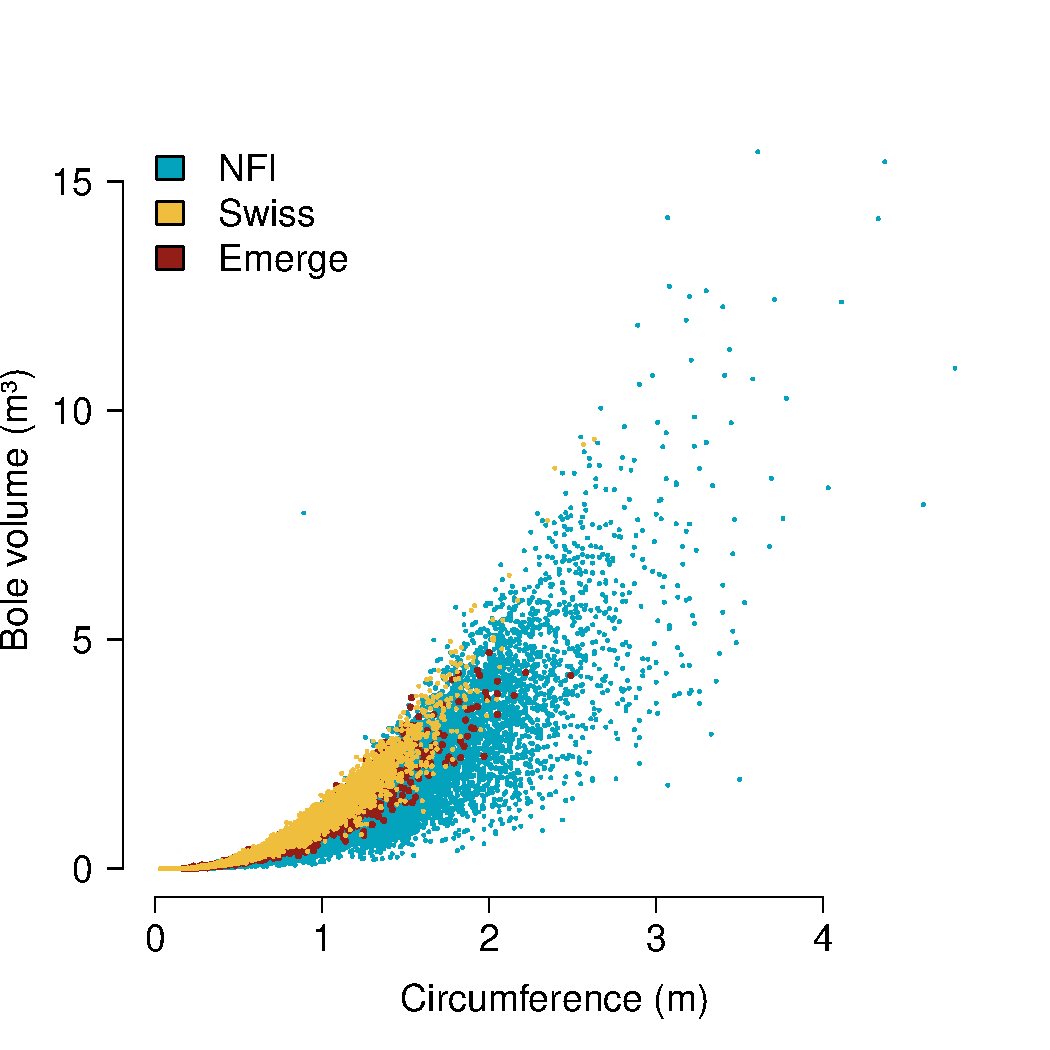
\includegraphics[scale = 0.4]{Figures/resp_fagus.pdf}
	\caption{Typical response of bole volume to circumference (here displayed for \textit{Fagus sylvatica}). We can see that both the Emerge and Swiss datasets \parencite{Deleuze2013,Didion2024} are quite similar and covers elongated trees, while the French \NFI{} covers less regular trees. \label{fig::fagSyl}}
\end{figure}

\begin{tcolorbox}[breakable, title = Bole volume (volume bois-fort tige)]
	The bole volume is the `reference' volume since the creation of the French \NFI{} (1958). Its definition is largely driven by the requirements of the wood industry, for which the estimation of standing timber volume is an essential tool for resource management and planning.
\end{tcolorbox}

\section{Notations}

We gather in the table \ref{tab::notations} the notations and acronyms used in this document.
\begin{table*}[h]
	\centering
	\begin{tabular}{@{}rp{10cm}l@{}}
		\toprule
		\multicolumn{1}{c}{\textbf{Symbol}} & \multicolumn{1}{c}{\textbf{Definition}} & \multicolumn{1}{c}{\textbf{Unit}} \\
		\( c \) & Circumference at breast height & \si{\centi\metre} \\
		\( h \) & Total tree height & \si{\metre} \\
		\( \hdec \) & Height to the stem top \( h \) or to a sharp narrowing (\( \geqslant 10\% \) decrease within \qty{1}{\metre}) & \si{\metre} \\
		\( \E[] \) & Expected value operator & diverse \\
		\EFM & Experimental Forest Monitoring \parencite{Didion2024} & - \\
		Emerge & Emerge project or dataset \parencite{Deleuze2013} & - \\
		\NFI & (French) National Forest Inventory & - \\
		\( r \) & Ratio of bole volume over total above-ground volume & - \\
		\( X, \, Y \) & Explanatory and dependent variables, \textit{resp.} & - \\
		\( \Vbole \) & Bole volume & \si{\cubic\metre} \\
		\( \Vtot \) & Total above-ground volume & \si{\cubic\metre} \\
		\( \alpha, \, \beta, \, \gamma \) & Parameters & diverse \\
		\( \symbfup{\theta} \) & Vector of parameters & diverse \\
		\( \mu \) & Mean parameter (often a function of explanatory variables and parameters) & - \\
		\( \phi \) & Precision of the beta distribution & - \\
		\( \rho \) & Correlation parameter (between \num{-1} and \num{1}) & - \\
		\( \Sigmabf \) & Variance-covariance matrix for the multivariate model & diverse \\
		\bottomrule
	\end{tabular}
	\caption{Used notations, sorted by alphabetical order with Latin symbols first.\label{tab::notations}}
\end{table*}
